\begin{figure*}[tp]
\centering
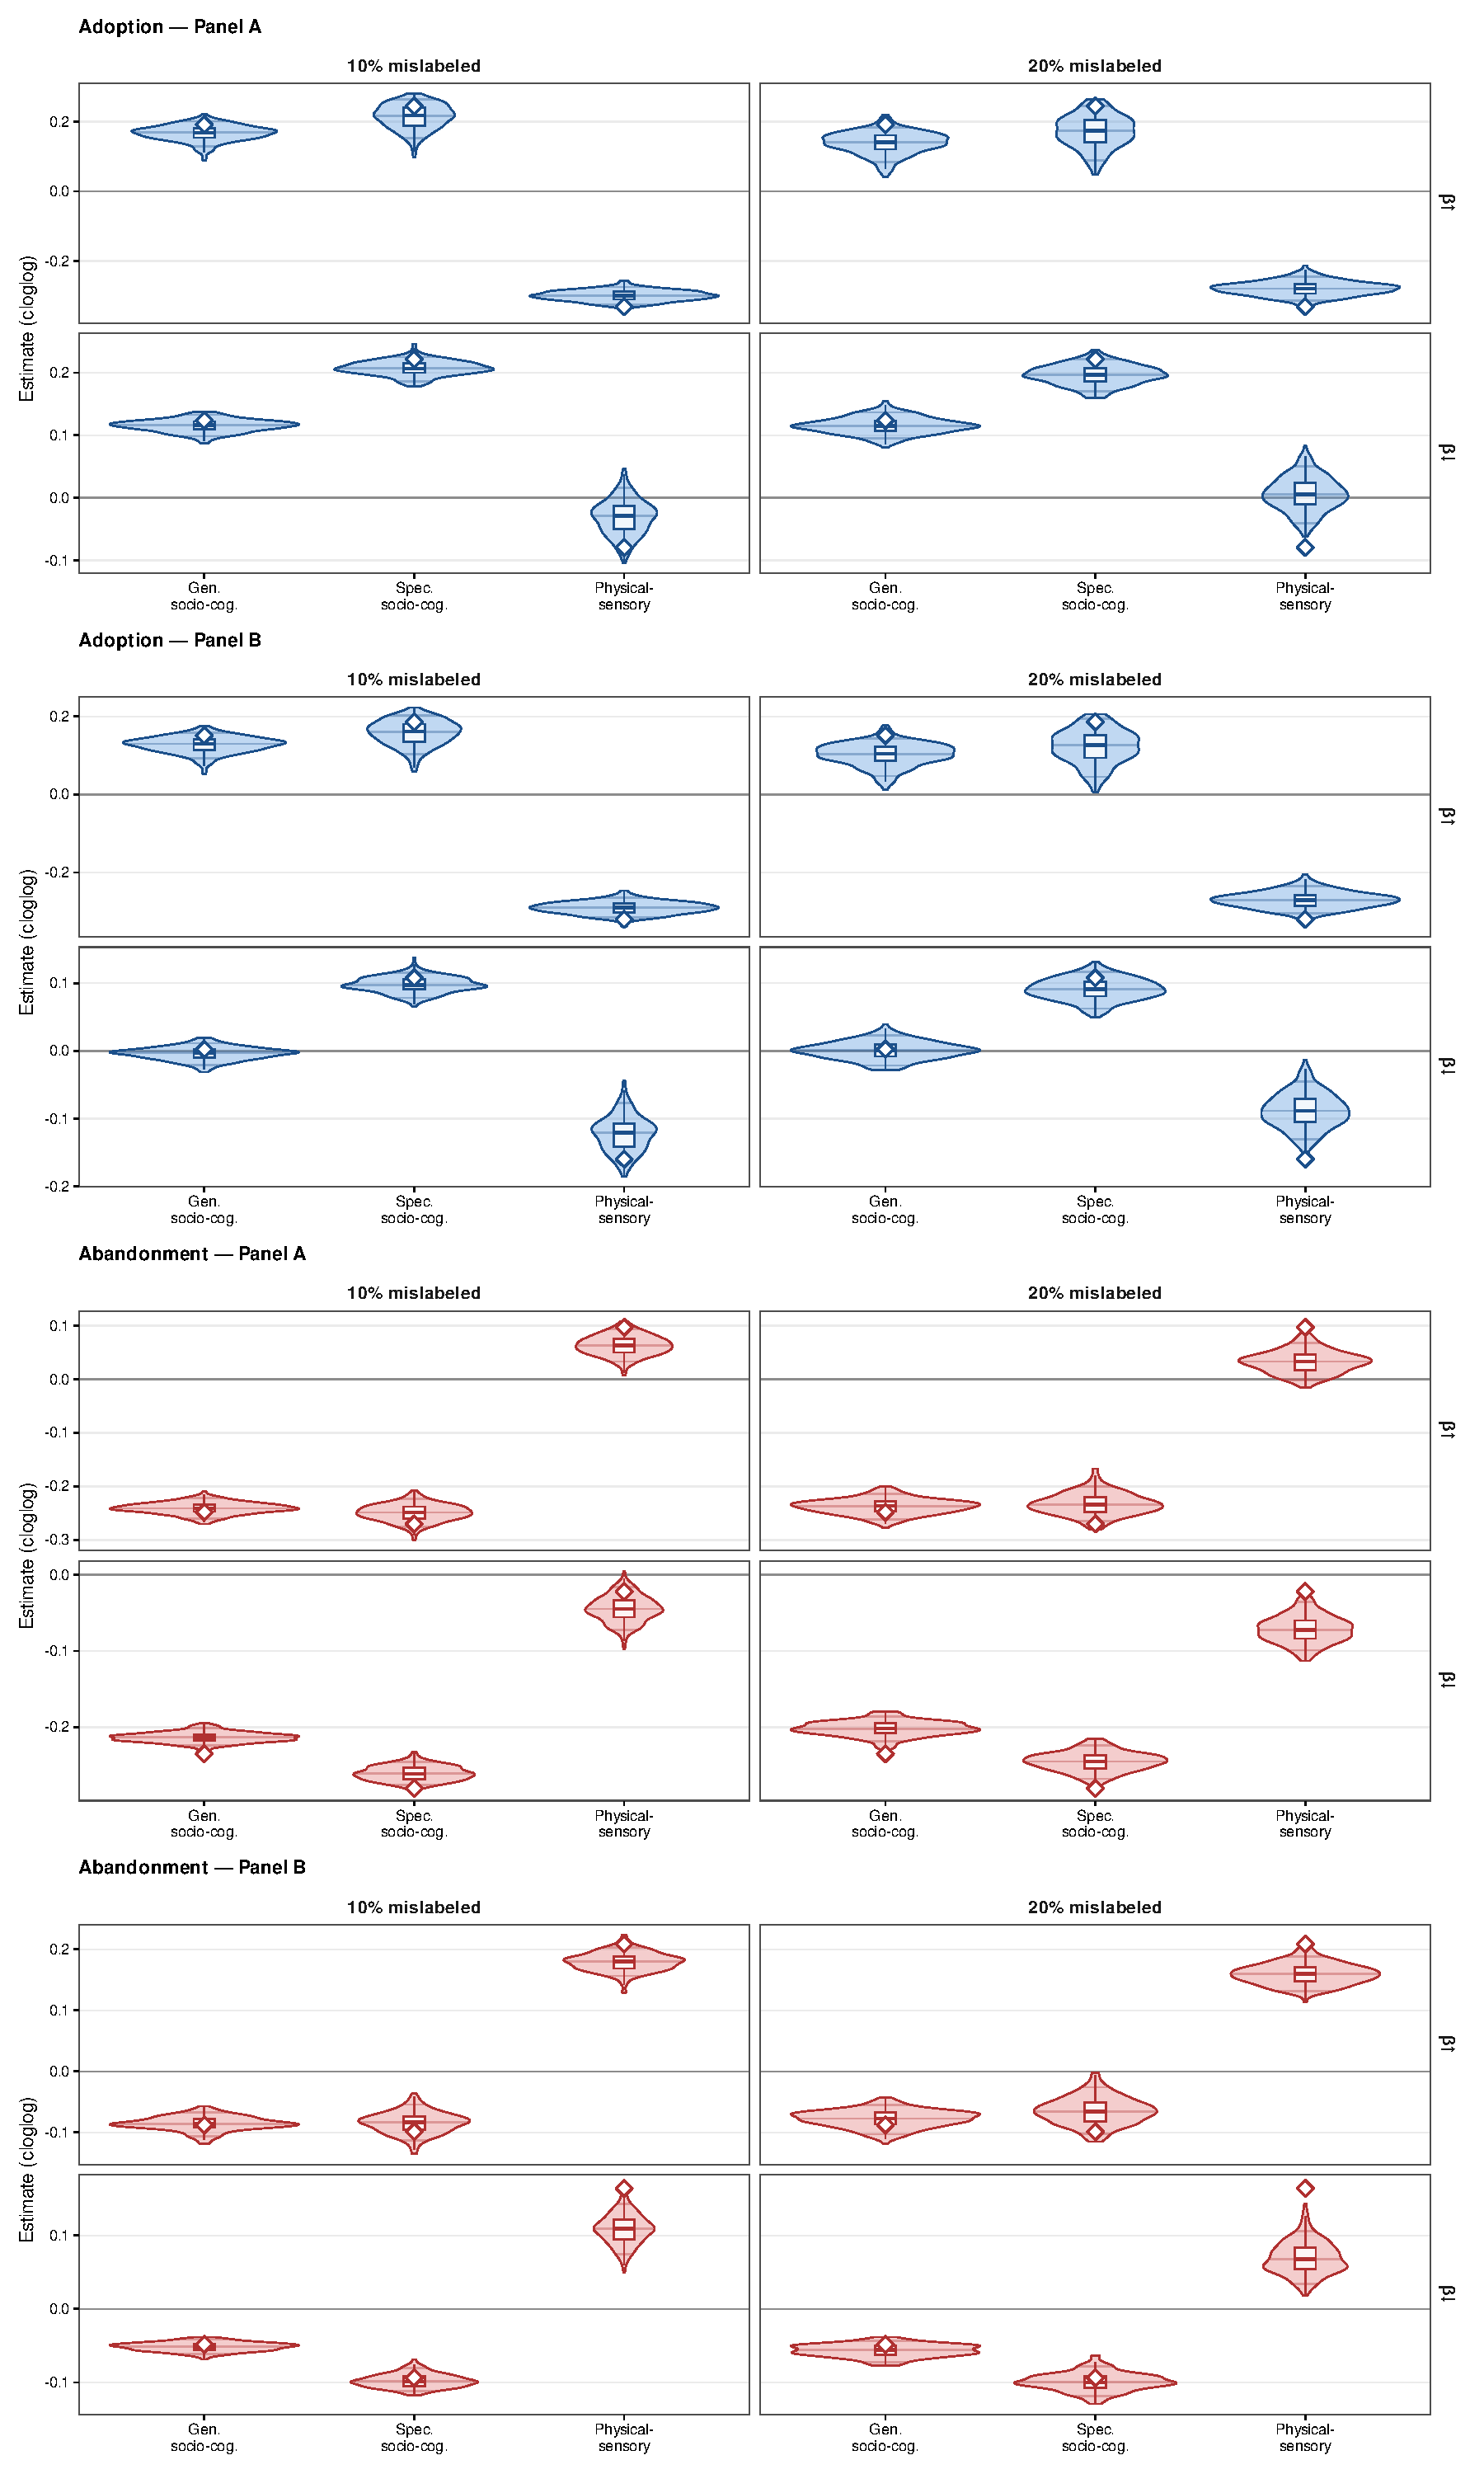
\includegraphics[width=0.75\textwidth]{figures/fig_archetype_misclassification.pdf}
\caption{\textbf{Directional gravity estimates are robust to skill-archetype misclassification.} Each violin shows the distribution of $\hat{\beta}^{\uparrow}$ (top row) and $\hat{\beta}^{\downarrow}$ (bottom row) across $B = 200$ replications in which a random fraction $p$ of skills is reassigned to a new archetype drawn from the empirical marginal distribution. Columns distinguish contamination levels (10\% and 20\% mislabeled); rows within each section distinguish $\hat{\beta}^{\uparrow}$ and $\hat{\beta}^{\downarrow}$. Internal lines in each violin mark the 5th, 50th, and 95th percentiles; the superimposed boxplot shows the interquartile range. Sections correspond to the four flow $\times$ fixed-effect combinations: Adoption Panel~A (blue, top), Adoption Panel~B (blue), Abandonment Panel~A (red), Abandonment Panel~B (red, bottom). Sign preservation exceeds 93.5\% in all 24 combinations and equals 100\% in 23 of 24. O*NET 2015--2024.}
\label{fig:SI_missclass}
\end{figure*}
